\documentclass[xcolor=pdftex,t,11pt]{beamer}


\usepackage{tipa}

\usetheme[
pagecounter=true,
pageofpages=of,  % page 7 "of" 9
bullet=circle,
titleline=true,
alternativetitlepage=true,
titlepagelogo=images/oxford_big_square,
% titlepagefooterlogo=images/oxford_small_square,
ordinarypageslogo=images/oxford_small_square,
% watermark=images/oxford_small_square,   % bottom right corner
% watermarkheight=100pt,
% watermarkheightmult=4,
]{Torino}
\usecolortheme{greenandblue}
\usefonttheme{structurebold}


\author{Volker Braun}
\title{Git and the New Sage Development Workflow}
\subtitle{Making distributed version control work for you}
\institute{Oxford University}
\date{September 23, 2013}

\begin{document}


\begin{frame}[plain]
	\titlepage
\end{frame}

\begin{frame}{Outline}
	\tableofcontents
\end{frame}



\subsection{Introduction}

\begin{frame}[fragile]
  \frametitle{Linguistic Approach}
  \vspace{-5mm}
  
  \begin{block}{}
    git \textipa{/gIt/}\\
    \textit{v Appalachian \& southern US}\\
    \hspace{1cm} variant of \emph{get}\\
    \textit{n Brit slang pejorative}\\
    \hspace{1cm} foolish or worthless person
  \end{block}
  \bigskip
  \pause

  \small
\begin{verbatim}
GIT(1)                   Git Manual                   GIT(1)

NAME
       git - the stupid content tracker

SYNOPSIS
       git [--version] [--help] [-c <name>=<value>]
           [--exec-path[=<path>]] [--html-path] [--man-path]
           ...
\end{verbatim}

\end{frame}


\begin{frame}
  \frametitle{Git, the DVCS}

  \begin{itemize}
  \item 
    Developed in 2005 to manage the Linux source code
    \begin{quote}
      I'm an egotistical bastard, and I name all my projects after
      myself. First ``Linux'', now ``git'' -- Linus Torvalds
    \end{quote}
  \item Slated to overtake \emph{Subversion} as the most popular VCS
    this year.
  \item \textbf{D}istributed -- there is no central server
  \item \textbf{V}ersion \textbf{C}ontrol \textbf{S}ystem -- manage
    changes to documents
  \item Git is free and open: \url{http://git-scm.com}
  \item Official \texttt{git} implementation: command-line program
  \item Various graphical user interfaces; I like \cmd{gitg} and \cmd{git-cola}
  \item Various websites offer git hosting (Github, Bitbucket,
    Mathematical Institute \url{https://git.maths.ox.ac.uk})
  \end{itemize}

\end{frame}



\begin{frame}
  \frametitle{Demo}
  
  Introduce the following commands:
  \begin{itemize}
  \item 
    Copy repository from github:\\
    \cmd{git clone}
    \\\hfill
    \cmd{https://github.com/vbraun/talk-git-sage-workflow.git}
  \item View history:\\
    \cmd{git log}
  \item Show current branch:\\
    \cmd{git branch}
  \item Switching between branches:\\
    \cmd{git checkout master}\\\cmd{git checkout my\_branch}
  \end{itemize}
\end{frame}



%%% Local Variables:
%%% TeX-master: "talk.tex"
%%% eval: (TeX-PDF-mode 1)
%%% End:



\begin{frame}[plain]
  \frametitle{Git Operations}
  \centering
  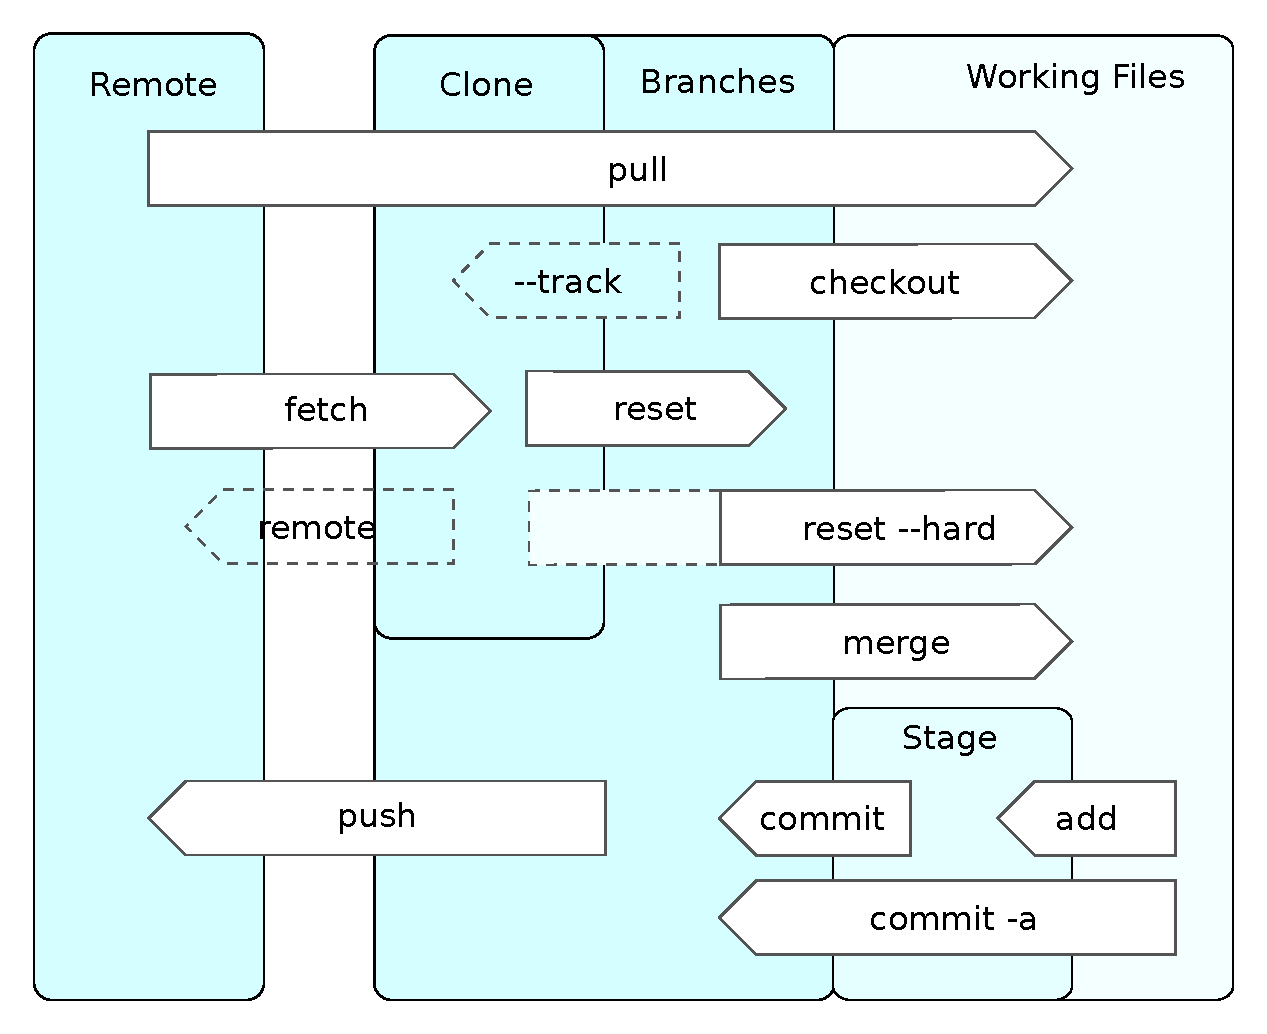
\includegraphics[width=0.85\linewidth]{images/git_operations}
\end{frame}


\end{document}


%%% Local Variables:
%%% eval: (TeX-PDF-mode 1)
%%% End:
